\documentclass[12pt,aspectratio=169]{beamer}

\usetheme{metropolis}

\definecolor{mDarkBrown}{HTML}{FF5722}
\definecolor{mDarkTeal}{HTML}{263238}
\definecolor{mLightBrown}{HTML}{FF5722}

\usepackage{booktabs}
\usepackage{graphicx}
\usepackage{hyphenat}
\usepackage{multirow}
\usepackage{nicefrac}
\usepackage[normalem]{ulem}

\usepackage{pifont}
\newcommand{\cmark}{\ding{51}}
\newcommand{\xmark}{\ding{55}}

\usepackage{minted}
\usemintedstyle{tango}
\newminted[bash]{bash}{%
    autogobble,
    bgcolor=mDarkTeal!10,
    linenos
}
\newminted[py3]{python}{%
    python3,
    autogobble,
    bgcolor=mDarkTeal!10,
    linenos
}
\newminted[sql]{sql}{%
    autogobble,
    bgcolor=mDarkTeal!10,
    linenos
}

\usepackage{polyglossia}
\setdefaultlanguage[variant=british]{english}
\usepackage[english=british]{csquotes}

\defaultfontfeatures{Ligatures=TeX}
\setmainfont{Lucida Sans OT}
\setsansfont[Scale=MatchLowercase]{Lucida Sans OT}
\setmonofont[Scale=MatchLowercase]{Lucida Console DK}

\usepackage{mathspec}
\setmathsfont(Digits,Latin,Greek)[Numbers={Lining,Proportional}]{Lucida Bright Math OT}

\newcommand{\mat}[1]{\ensuremath{\mathbf{#1}}}

\newcommand{\R}{\ensuremath{\mathbb{R}}}

\newcommand{\E}[1]{\ensuremath{\mathbb{E}\!\left[ #1 \right]}}
\newcommand{\V}[1]{\ensuremath{\mathbb{V}\!\left[ #1 \right]}}
\newcommand{\Prob}[1]{\ensuremath{\Pr\!\left( #1 \right)}}
\newcommand{\Normal}[2]{\ensuremath{\mathcal{N}\!\left( #1, #2 \right)}}
\newcommand{\simiid}{\ensuremath{\overset{\text{\tiny i.i.d.}}{\sim}}}

\DeclareMathOperator{\logit}{logit}

\author{Gianluca Campanella}
\date{}



\title{Epilogue}

\begin{document}

\maketitle

\begin{frame}{Contents}
    \tableofcontents[hideallsubsections]
\end{frame}

\section{Use the right tools for the job}

\begin{frame}{What is Data Science?}
    \begin{center}
        \LARGE%
        A \alert{problem\hyp{}solving approach} \\
        based on the scientific method
    \end{center}
\end{frame}

\begin{frame}{Use the right tools for the job}
    \begin{center}
        \Large%
        Remember that the focus is on \alert{adding value}
    \end{center}
    \vfill
    \begin{itemize}
        \item[$\rightarrow$] Find and use the right tools for the job
        \item Even if it happens to be Excel!
    \end{itemize}
\end{frame}

\begin{frame}{Don't try to run before you can walk}
    \begin{center}
        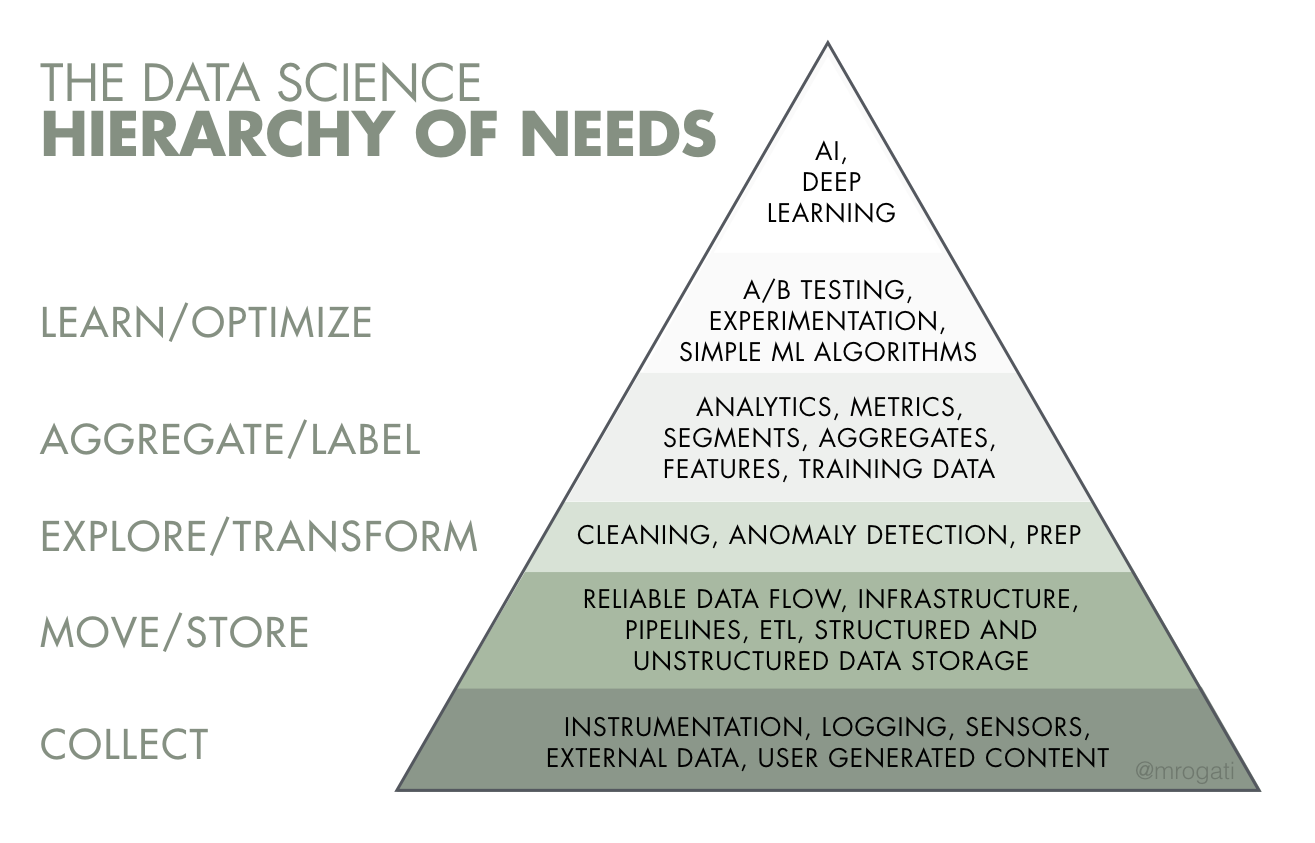
\includegraphics[height=0.8\textheight]{figures/ai_hierarchy} \\
        {\scriptsize%
         From M.\ Rogati}
    \end{center}
\end{frame}

\begin{frame}[fragile]{Machine Learning models}
    \begin{center}
        \renewcommand{\arraystretch}{2}
        \begin{tabular}{cr|cc}
                &                       & \textbf{Categorical} & \textbf{Numerical} \\ \hline
                & \textbf{Supervised}   & \parbox[c]{3cm}{\centering Classification} & \parbox[c]{3cm}{\centering Regression} \\
                & \textbf{Unsupervised} & \parbox[c]{3cm}{\centering Clustering}     & \parbox[c]{3cm}{\centering Dimensionality\\[-\smallskipamount]reduction} \\
        \end{tabular}
    \end{center}
\end{frame}

\section{Don't fool yourself}

\begin{frame}{Don't fool yourself}
    \begin{center}
        \Large%
        It's only numbers after all!
    \end{center}
    \vfill
    \begin{itemize}
        \item There is no causation without manipulation
        \item If it sounds too good to be true\ldots
    \end{itemize}
\end{frame}

\begin{frame}[t]{Bias\hyp{}variance trade\hyp{}off}
    \begin{itemize}
        \item \alert{Irreducible variance} due to the stochastic process
        \item \alert{Bias} in approximating $f^{\,\star}$ using $f$
        \item \alert{Estimation variance} of $\hat{f}$
    \end{itemize}
    \vfill
    \begin{center}
        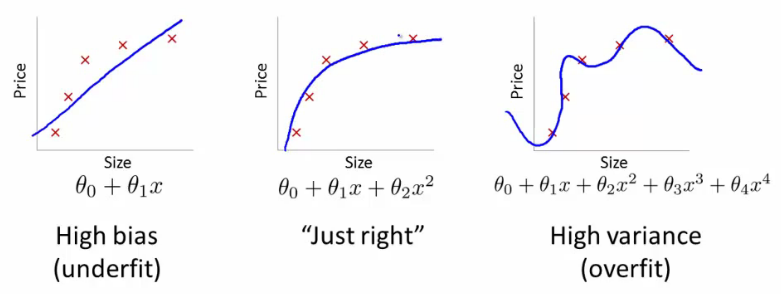
\includegraphics[width=0.8\textwidth]{figures/underfitting_overfitting} \\
        {\scriptsize%
         (From Andrew Ng's ML course)}
    \end{center}
\end{frame}

\begin{frame}{Bias\hyp{}variance trade\hyp{}off and generalisability}
    \begin{center}
        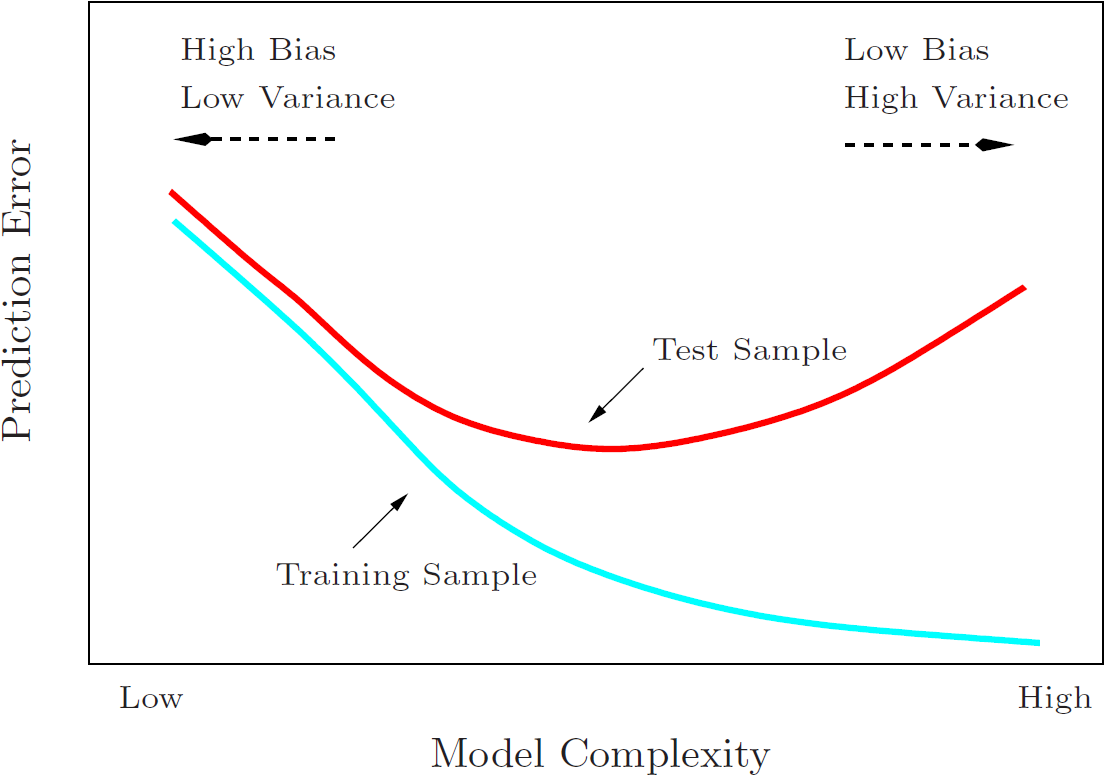
\includegraphics[height=0.8\textheight]{figures/generalisability} \\
        {\scriptsize%
         From \textit{The Elements of Statistical Learning}}
    \end{center}
\end{frame}

\section{Don't be evil}

\begin{frame}{Don't be evil}
    \begin{center}
        \Large%
        The biggest threat is not from AI\ldots

        \vfill\pause

        \ldots but from the humans who control it
    \end{center}
\end{frame}

\end{document}

